\chapter{Analyse}
%Evaluation der SAP Business Technology Platform für die Anforderungen auf dem deutschen Kfz-Versicherungsmarkt
\section{Task Charakteristiken - Identifikation der Anforderungen der Kfz-Versicherer an digitale Plattformen}

\subsection{Literaturbetrachtung aktueller Anforderungen an digitale Plattformen}

\begin{figure}[h]
    \centering
    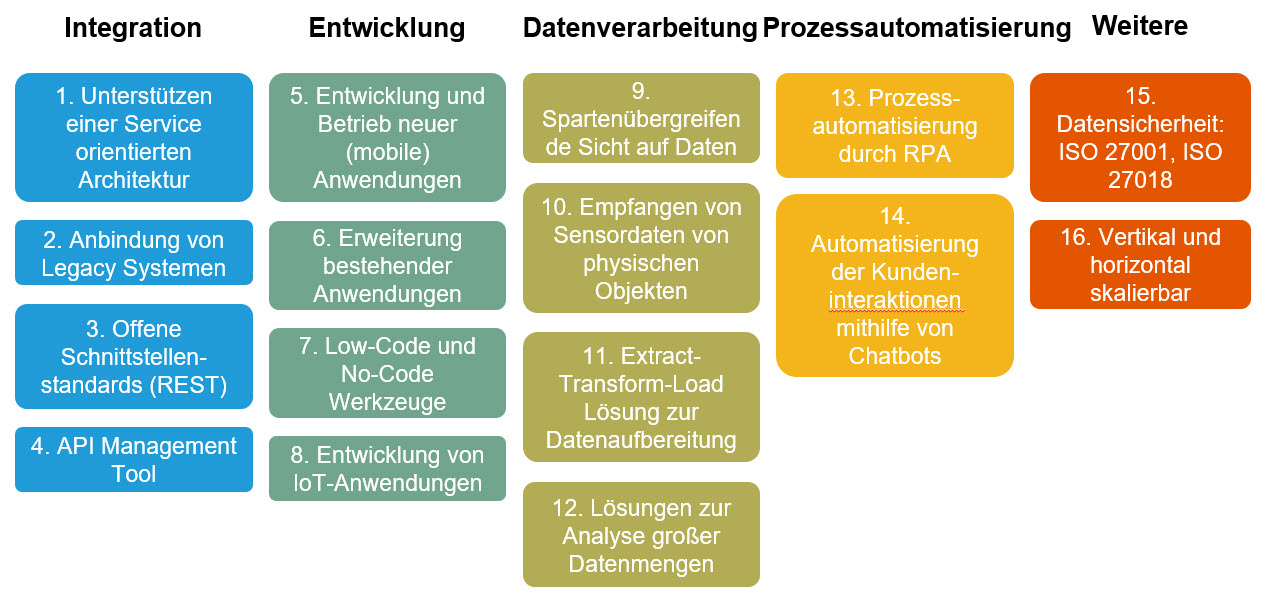
\includegraphics[width=1\textwidth]{img/PP_Anforderungen.jpg}
    \caption[Anforderungen der Kfz-Versicherer an digitale Plattformen]{Anforderungen der Kfz-Versicherer an digitale Plattformen\autocite{PPAnf}}
    \label{fig:PPAnf}
\end{figure}
\footnotetext{eigene Darstellung}

Eine der größten Herausforderungen, denen sich Versicherungsunternehmen stellen müssen, sind die historisch bedingten IT-Landschaften, die auch als IT-Legacy oder Legacy-Systeme bezeichnet werden. Diese sind seit Beginn der 1970er Jahre entstanden und wurden dabei größtenteils von den Versicherern selbst entwickelt. Mittlerweile führt allerdings genau diese IT-Legacy aufgrund der starken Abhängigkeiten zwischen den Systemen und der monolithischen Programmstruktur häufig zu langen Entwicklungszyklen (vgl. S. 10-12 Gunter2020) (BAIN) Um dennoch adäquat auf die sich ändernden Kundenbedürfnisse und Marktbedingungen reagieren zu können, müssen Kfz-Versicherer eine neue technologische Plattform zur Neugestaltung ihrer IT-Landschaft einführen. Dabei sollte die Plattform eine Service-orientierte Architektur (SOA) unterstützen, damit bestehende, bereits abgeschlossene Software-Bausteine, wie zum Beispiel die Rechenkerne der verschiedenen Versicherungssparten, weiterhin genutzt und in die neue IT-Infrastruktur integriert werden können. (vgl. S. 10-11 Urlaß) Darüber hinaus erleichtert der modulare Aufbau einer SOA auch das Hinzufügen und Entfernen neuer Anwendungen an der Kundenschnittstelle.(BAIN)

Bei der Einführung einer neuen technologischen Plattform ist eine grundlegende Anforderung der Versicherungsunternehmen, die Anbindung der bestehenden Legacy-Systeme, da diese eng mit den bestehenden Geschäftsprozessen verknüpft sind und Daten enthalten, welche aus regulatorischen Gründen noch aufbewahrt werden müssen. Hierfür können im Rahmen einer SOA die einzelnen, logischen Elemente der Systemlandschaft isoliert und anschließend mithilfe einer (SOAP)-Schnittstelle als Service den anderen Systemen zur Verfügung gestellt werden. Daher muss eine technologische Plattform für Kfz-Versicherer das Simple Object Access Protocol unterstützen. (vgl. GUNTER2020 S. 10-12)

Darüber hinaus sollte es die Plattform ermöglichen, bestehende Anwendungen mithilfe von kleinen Programmcodes eigenständig erweitern zu können, um die Anwendungen nach den Bedürfnissen der Kfz-Versicherer anpassen zu können. Hierbei gilt es zu berücksichtigen, dass insbesondere bei kleinen und mittelgroßen Versicherern die Entwicklungsressourcen sehr knapp sind. Daher sollte die Plattform ebenfalls sogenannte Low- oder besser No-Code-Werkzeuge bereitstellen, damit auch Nutzer aus den Fachabteilungen Erweiterungen erstellen können.(3) (vgl. WEINGARTNER2023)

Eine Trend der insbesondere in den nächsten Jahren die Versicherungsbranche bestimmen wird, sind die sogenannten Digitalen Ökosysteme und die damit verbundenen Partnerschaften. So erachten gemäß einer Studie der Swiss RE aus dem Jahr 2019 mehr als 75\% der Führungskräfte von Versicherungsunternehmen weltweit digitale Ökosysteme und andere Partnerschaften als wesentlich für die Schaffung von Wettbewerbsvorteilen. (vgl. PAYNE2022) (vgl. AVRAMAKIS2023) Für die Partizipation an Digitalen Ökosystemen ist dabei vor allem das Vorhandensein offener Standardschnittstellen und Austauschformate maßgebend, sodass ähnlich wie im Banking mit der PDS2 Richtlinie auch Versicherungsunternehmen ihre Daten leicht mit Partnern und Drittanbietern  teilen können. Zu diesem Zweck hat sich 2018 (vgl. 2021z) die Free Insurance Data Initiative (FRIDA)  gebildet, welche für die einzelnen Versicherungssparten offene Schnittstellen Standards schaffen möchte. In der in der Kfz-Versicherungssparte ist es die sogenannte Car-ClaimsAPI, welche als REST-Schnittstelle den Austausch von Kfz-Police Daten vereinfachen soll. Folglich sollte eine Plattform für Kfz-Versicherer auch Rest-API-Calls unterstützen, um sich mit Partnern und InsurTechs in einem Digitalen Ökosystem verbinden zu können und somit wettbewerbsfähig zu bleiben. (vgl. KRETZ2023) 

Zudem wird es immer wichtiger, nicht die Kontrolle und Übersicht über die einzelnen Schnittstellen zu verlieren, insbesondere dann, wenn alter Code der nie für eine Internet-Anbindung ausgelegt war, mit einem Mal öffentlich zugänglich wird. (vgl. B. S.137) (S.393 HANSCHKE2021) Daher sollten technologische Plattformen für Kfz-Versicherer über eine API-Management-Tool verfügen, um die API-Aufrufe in und außerhalb der Unternehmens analysieren, kontrollieren und verwalten zu können. (vgl S.83fHANSCHKE2021)

Darüber hinaus zeigt sich die Herausforderung der Legacy-Systeme auch im Datenmanagement. So existieren in den fragmentierten IT-Landschaften viele firmeninterne Datensilos, die keine integrierte Sicht auf die Daten erlaubt. Um diese Herausforderung zu überwinden sollte die technische Plattform eine spartenübergreifende Sicht auf alle Daten ermöglichen. (vgl. GUNTER2020 S. 11)

Daneben ist es im Rahmen des Datenmanagements wichtig sicherzustellen, dass die Daten in einem konsistenten und strukturierten Format vorliegen, sodass auf dieser Grundlage eine effektive Analyse und Verwaltung der Daten möglich ist. Folglich muss die Plattform eine Extract-Transform-Load (ETL)-Lösung bereitstellen, um Daten aus verschiedenen Quellen zu extrahieren, sie zu transformieren und schließlich in ein Zielsystem zur Analyse laden zu können. (vgl. WEINGARTNER2023), (vgl. ASCHENBRENNER2010 S. 342-345)

Durch die Technologisierung der Automobilbranche und den umfangreichen Daten, die in Fahrzeugen erhoben werden, hat sich die Kfz-Versicherung als Vorreiter der Assekuranz im Bereich Data Analytics hervorgetan.(vgl. GATZERT2023 S. 230) Die Auswertung von großen vernetzten Datensätzen, auch als Big Data bezeichnet, ermöglicht eine genauere Abschätzung bestehender Risiken und führt somit zu einer exakteren Kalkulation von Prämien und neuen Produkten. Dies ist auf die Anwendung der Wahrscheinlichkeitstheorie zur Prämienberechnung zurückzuführen, bei der ein höheres Ausmaß an untersuchten Fällen zu einem präziseren Ergebnis führt. Daher sollte eine technologische Plattform für Kfz-Versicherungen auch Lösungen zur Analyse großer Datenmengen bieten, um den Kfz-Versicherern eine optimale Prämien- und Risikokalkulation zu ermöglichen (vgl. MANGEI 2019 S. 146).

Des Weiteren wird das von einem Menschen gesteuerte KFZ immer selbstständiger und vernetzter, bis hin zu autonom verkehrenden Fahrzeugen. Dies hat zu einer Zunahme von Telematik-Tarifen in der Branche geführt, wobei eine Studie von Roland Berger aus dem Jahr 2015 prognostiziert, dass bis 2030 etwa 25\% des Kfz-Versicherungsmarktes von Telematik-Produkten dominiert werden (vgl. ROLANDBERGER 2015 S.4) \improvement{Aktualität: Studie ist älter 2030 an 2023 ist} Telematik bezeichnet allgemein die Verbindung von Informatik und Telekommunikation, (vgl. ABTS2017 S. 10-11) und ermöglicht in der Kfz-Versicherungsbranche die Berücksichtigung des individuellen Fahrverhaltens des Versicherungsnehmers sowie anderer externer Rahmenbedingungen bei der Prämienermittlung.(vgl. MERZINGER2017 S.84) So kann der Versicherer seine Produkte besser an das Risikoprofil seiner Kunden anpassen und die Kunden bei einer zurückhaltenden Fahrweise von günstigeren Preisen profitieren. Hierfür werden mithilfe von Sensoren im Auto verschiedene Daten zum Fahrstil des Nutzers erfasst und zur Prämienermittlung an der Versicherer übermittelt.(vgl. ELING2020 S. 3-4) Für den Einsatz von technologischen Plattformen bei Kfz-Versicherern ist es folglich wichtig, dass die Plattform Sensordaten von physischen Objekten in Echtzeit empfangen und verarbeiten kann.(vgl. Link zu: Das Kfz, die Telematik und der Datenschutz S. 10-15) Zudem sollte die Plattform auch Möglichkeiten zur Entwicklung von IoT-Anwendungen bereitstellen, um Sensordaten in Geschäftsprozesse integrieren zu können.

Neben den bestehenden Legacy-Systemen und der Wertschöpfung aus Daten, haben zahlreiche Kfz-Versicherer mit dem Problem zu kämpfen, dass viele ihrer internen repetitiven Prozesse noch manuell von Mitarbeitern ausgeführt werden müssen. Dies führt zu langen Bearbeitungszeiten, Anfälligkeit für menschliche Fehler und einer Bindung von wertvollem Humankapital, das nicht für die Kundenbetreuung eingesetzt werden kann. Eine Lösung zur Bewältigung dieser Herausforderung, die auch von der technologischen Plattform unterstützt werden sollte, ist die Robotic Process Automation (RPA). So können durch RPA repetitive Aufgaben wie beispielsweise die Übertragung von Daten in Systeme, das Erstellen von Berichten oder das Überprüfen von Schäden automatisiert werden. Die Allianz vermutet, dass durch den Einsatz von RPA, die Arbeitszeit um 40\% reduziert und gleichzeitig die Qualität der Leistung verbessert werden. Dies betont noch einmal die Bedeutung von RPA für die Wettbewerbsfähigkeit in der Branche. (vgl. REICH2019 S. 296-298)

Gemäß Reich (2019) besteht eine zusätzliche Option für die Automatisierung von Kundeninteraktion in Fällen wie Anträgen, Auskünften oder Schadensmeldungen durch den Einsatz von Chatbots. So können Fragen von Kunden, insbesondere solche, die sich auf Versicherungspolicen, Abrechnungen oder Schadensmeldungen beziehen, jederzeit beantwortet werden, ohne dass der Kunde auf einen Mitarbeiter warten muss. Dadurch kann der Bedarf nach Mitarbeitern in der Sachbearbeitung reduziert und die Kundenzufriedenheit erhöht werden, weshalb die Plattform für Versicherer auch Chatbot-Funktionalitäten bereitstellen sollte. (vgl. REICH2019 S. 300-302)

Des Weiteren ist das Smartphone und die damit verbundenen Anwendungen ein ständiger Begleiter der Versicherungsnehmer. Dabei können die Anwendungen im Kfz-Versicherungskontext beispielsweise bei einem Autounfall genutzt werden, um den eigenen Standort sowie Fotos vom Schaden zu teilen. Folglich ist die Unterstützung mobiler Anwendung eine Anforderung für die Verwendung einer technologischen Plattform in der Kfz-Versicherungsbranche. (vgl. BAIN2013 S.16)

Aufgrund der strengen regulatorischen Anforderungen in der Versicherungsbranche ist die Datensicherheit eine Grundvoraussetzung für jegliche eingesetzte Softwarelösung und somit auch für technische Plattformen. Dabei ist die Bewertung des Sicherheitsniveaus einer Software mühsam und zeitaufwendig, weshalb Versicherungsunternehmen in der Praxis auf Zertifizierungen und Testate zurückgreifen. (vgl. ZDANOWIECKI2016 S. 777) Bei cloud-basierten Lösungen gilt dabei die ISO/IEC 27001 Norm als  Standard, da sie die Anforderungen an ein Informationssicherheitsmanagementsystem (ISMS) definiert. Darüber hinaus müssen Kfz-Versicherer sicherstellen, dass die Verarbeitung von Daten den Bestimmungen der Datenschutzgrundverordnung (DSGVO) entspricht, um den Schutz personenbezogener Daten zu gewährleisten. Zu diesem Zweck wurde im Jahr 2014 der ISO/EIC 27018-Standard speziell entwickelt. Daher sollten technische Plattformen für Kfz-Versicherer sowohl nach ISO/EIC 27001 als auch nach ISO/EIC 27018 zertifiziert sein.

Eine weitere Anforderung, die ebenfalls von Beginn an erfüllt sein sollte, ist die Fähigkeit der Plattform zur horizontalen und vertikalen Skalierbarkeit. Dies erfordert, dass die Plattform zusätzliche Server automatisch starten und Lasten auf mehrere Server verteilen kann, um plötzliche und hohe Nutzerzahlen zu bewältigen, wie sie zum Beispiel im Herbst bei Kfz-Versicherungen vorkommen können. (horizontale Skalierbarkeit). Des Weiteren muss die Plattform in der Lage sein, je nach Bedarf die Rechenleistung und Speicherkapazität des Servers zu erhöhen, um einem höheren Ressourcenbedarf gerecht zu werden (vertikale Skalierbarkeit). (vgl. JAHNERT2020 S. 23)

Eine tabellarische Auflistung der Anforderungen ist dem Anhang ... zu entnehmen. (kommt noch)











\subsection{Evaluation und Ergänzung der Anforderungen aus Sicht der Experten}

Die zuvor aus der Literatur herausgearbeiteten Anforderungen konnten von allen Experten bestätigt werden. Hervorgehoben wurde dabei insbesondere, dass der Preis für den Endkunden der alles entscheidende Faktor ist und daher aktuell alle Kfz-Versicherer versuchen, ihre komplette Lieferkette zu automatisieren. Dabei wurde ebenfalls die Unterstützung von mobilen Anwendungen als sehr wichtig betont, um dort dann beispielsweise Tätigkeiten wie das Buchen eines Werkstatttermins durchzuführen. Des Weiteren wurde von Experte 1 das Unterstützen einer „Entkopplungsarchitektur“ als Anforderung genannt, damit Kfz-Versicherer agil an der Kundenschnittstelle agieren und gleichzeitig auf die statischen Informationen aus den Altsystemen zugreifen können. Die dafür notwendige Kapselung der Altsysteme und das Bereitstellen dieser über Schnittstellen entspricht im wesentlichen einer SOA. Zudem wurde von Experte 2 die leichte Integration der Kfz-Versicherer in Ökosysteme und Vertriebskanäle wie Check24 mit den Schlagworten Open und Embedded Insurance betont. Beide werden im Rahmen dieser Arbeit unter der Anforderung offene Schnittstellenstandards zusammengefasst, da diese die dafür notwendige Voraussetzung sind. Weitere Anforderungen die von den Experten ergänzt wurden, werden im Folgenden kurz vorgestellt.

17. Entscheidungsfindung durch KI. – Für Experte 2 stellte zudem eine weitere Anforderung das Unterstützen der Kfz-Versicherer bei der Entscheidungsfindung durch KI Modelle in Prozesse wie der Akquise oder dem Schadensprozess dar, um bestimmte Sachverhalte prüfen zu lassen.

18. Bereitstellung einer Prozessorchestrierungslösung – Aus Sicht des Experten 3 ist es für Kfz-Versicherer zudem wichtig ein Prozessorchestrierungstool zu haben, um einen Prozess systemübergreifend end-to-end designen und gezielt Prozessschritte in den jeweiligen Lösungen über Schnittstellen ansteuern zu können.

19. Wenig Wartungsaufwand – Für Experte 3 stellte eine weitere grundlegende Anforderung die einfache Wartbarkeit der Plattform dar, sodass beispielsweise neue Releases automatisch eingespielt und damit die neuesten Technologien direkt bereitgestellt werden.

20. Contentpakete – Aus Sicht des Experten 3 sollte eine technische Plattform neben den bereitgestellten Tools in den einzelnen Clustern auch Contentpakete bereitstellen. Mit dem Begriff Content sind dabei Inhalte gemeint, die den Implementierungsaufwand in den einzelnen Bereichen reduzieren. Das können bspw. vordefinierte Schnittstellen, Adaptoren, vordefinierte Datenmodelle oder auch vordefinierte Frameworks sein. 

Neben der Überprüfung und Ergänzung der in der Literatur gefundenen Anforderungen, wurden diese von den Experten ebenfalls nach ihrer Wichtigkeit in den nächsten 3-5 Jahren priorisiert. Diese Priorisierung ist in Tabelle  … dargestellt.

\begin{figure}[h]
    \centering
    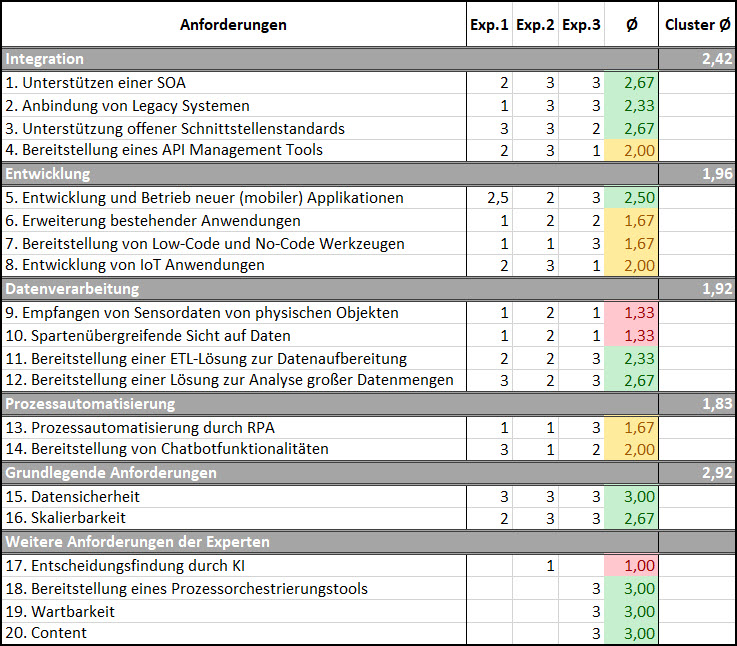
\includegraphics[width=1\textwidth]{img/Gewichtung_Anforderung.jpg}
    \caption[Gewichtung der Anforderungen durch die Experten]{Gewichtung der Anforderungen durch die Experten\autocite{Gewichtung}}
    \label{fig:Gewichtung}
\end{figure}
\footnotetext{eigene Darstellung}

Anhand der Tabelle ist zu erkennen, dass die Experten die einzelnen Anforderungen zwar teilweise sehr unterschiedlich bewerten, sich aber dennoch einige Tendenzen erkennen lassen. So sind neben den grundlegenden Anforderungen insbesondere die Anforderungen im Bereich der Integration besonders wichtig. Darauf gefolgt sind mit einem Durchschnittswert von ca. 1,9 die Anforderungen im Bereich der Entwicklung und im Bereich der Datenverarbeitung für in etwa gleichwichtig befunden worden. Die Anforderung im Cluster der intelligenten Technologien sind nach Einschätzung der Experten am wenigsten wichtig.















\section{Technologie Charakteristiken - Komponenten und Services der SAP Business Technology Platform}\label{sec:TechCharak}

Nachdem die Task Charakteristiken mithilfe einer systematischen Literaturanalyse sowie mit Experteninterviews ermittelt wurden, werden nachfolgend die Charakteristiken der SAP BTP  der SAP BTP beschrieben.  Diese bauen auf den sogenannten Foundational Services der SAP BTP auf und lassen grundlegend in die Bereiche: Datenbank und Datenbankmanagement, Datenanalyse, Anwendungsentwicklung, Integration sowie Intelligente Technologien unterteilen.

Da die Plattform sehr viele Services in den einzelnen Bereichen umfasst wird sich im Rahmen dieser Arbeit in jedem Bereich auf die Kernfunktionalitäten beschränkt, um den Umfang der Arbeit nicht zu übersteigen.

Grundsätzlich lässt sich dabei festhalten, dass die Services der einzelnen Bereiche als Cloud Service konsumiert werden und Cloud-Eigenschaften wie Elastizität, Skalierung und Hochverfügbarkeit ermöglichen. (vgl. Seubert S. 60)
** hier auch die neben der Skalierbarkeit ebenfalls die Sicherheit einbauen.
Abbildung aus S. 59 einbauen

Die gemeinsame technische Basis der Plattform Services ist in Abbildung --- durch den Kasten Common Foundation und Services dargestellt. Hierzu gehören Dienste wie z.B. ein Identity Service zur Authentifizierung, ein Audit-Log-Service zum Aufzeichnen von sicherheitsrelevanten Handlungen, ein Application Autoscaler zur automatischen Skalierung von Anwendungen, sowie eine Pipeline Configuration für Continuous integration and delivery. (vgl. SEUBERT S. 58)

Im Bereich des Datenmanagements lassen sich mit der SAP BTP verschiedene Datenarchitekturen wie eine zentrale Datenplattform, ein Data Lake sowie eine Data Fabric realisieren. Für die transaktionale Verarbeitung von Daten stellt die BTP Datenbank Services wie SAP HANA Cloud zu Verfügung. Hier werden mithilfe von Konnektoren auch externe Datenquellen in eine zentrale Datenarchitektur entweder virtuell oder über eine Replikation integriert. Für die Verwaltung und Aufbereitung noch größerer Mengen strukturierter, halbstrukturierter und unstrukturierter Daten kann der SAP BTP Service Data Intelligence verwendet werden. Dieser stellt einen für Petabyte-Volumen ausgerichteten Data Lake bereit, mit dem Datensilos verknüpft und zusätzlich Machine-Learning-Modelle entwickelt werden können. Darüber hinaus können alle Aufgaben, die für eine Integration und Verarbeitung der Daten erforderlich sind, von dem Data Intelligence Service orchestriert werden.(vgl. DATAINTELLIGENCE) Darauf aufbauend können mit dem Service SAP Datasphere auch Data Fabric-Architekturen aufgebaut werden. (vgl. Seubert S. 60-63) Dadurch können bisher getrennte Funktionen zu einem einheitlichen Service für Datenintegration, Katalogisierung, Data Warehousing und Virtualisierung von Workloads für SAP- und Nicht SAP-Daten kombiniert werden. Das wiederum ermöglicht es, SAP- und Nicht-SAP-Cloud sowie on-Premise-Quellen, einschließlich Data Lakes zu verbinden, um die dort enthaltenen Daten zu föderieren, zu transformieren und in ein für die Auswertung/ Analyse zuständiges Zielsystem zu laden. (vgl. FSDDATASPHERE S.3-4) 

Object Store Service

Master Data Governance

Die Funktionalitäten und Services der SAP BTP zur Datenanalyse bauen auf den Services des Datenmanagements auf, da die Daten in einer strukturierten und transformierten Form vorliegen müssen, bevor sie analysiert werden können. Der zentrale Service im Bereich der Datenanalyse ist dabei die SAP Analytics Cloud. Diese ist ein SaaS Produkt für Business Intelligence und Analytics, welches die aufbereiteten Daten mithilfe Visualisierungen wie z.B. Charts, Tabellen oder Karten in Berichten (Stories) darstellt. (vgl. SAC) Dabei ermöglicht die Interaktion mit den Darstellungen (bspw. via Drill-Downs) den Fachbereichsnutzern es, weitere Erkenntnisse über einen Sachverhalt zu sammeln und durch das Verwenden von Filtern unterschiedliche Perspektiven und Schwerpunkte für eine zielgerichtete Interpretation zu setzen. Darüber hinaus können mit der SAC auch vielfältige Planungsszenarien wie beispielsweise eine Absatzprognose in Form von Tabellen aufgebaut werden. Dadurch können Nutzer beispielsweise analysieren, wie sich die verschiedenen Unternehmensbereiche gegenseitig beeinflussen.(vgl. Seubert S. 64-67)
Zudem können mit der Data Warehouse Cloud der BTP  Daten aus unterschiedlichen SAP und Nicht-SAP-Quellen über eine Datenintegration und ETL-Prozesse (Extract, Transform, Load) zentral zusammengeführt werden.

Neben dem Datenmanagement und der Datenanalyse stellt die SAP BTP ebenfalls Funktionalitäten für die Anwendungsentwicklung bereit, die unterschiedliche Abschnitte des Softwarelebenszykluses abdecken. Abhängig von den jeweiligen funktionalen Anforderungen, können die Anwendungen bzw. Erweiterung auf unterschiedlichen Laufzeitumgebungen entwickelt werden. Hierzu gehören die Cloud Foundry Runtime Environment zur Entwicklung von Microservices basierenden Erweiterungen, das SAP BTP ABAP Environment zur Entwicklung und Bereitstellung von ABAP Anwendungen, sowie SAP Kyma für containerbasierte Anwendungen und Erweiterungen. Darüber hinaus wird ebenfalls SAP BTP Neo Environment unterstützt, welches die Entwicklung von Erweiterungen von nativen SAP-HANA-Anwendungen ermöglicht. Zur Beschleunigung der Entwicklung werden mit dem SAP Cloud Application Programming Model (CAP) ein Framework für die Programmiersprachen Java und Node.js bereitgestellt. Zusätzlich werden von der SAP BTP mit dem sogenannten Mobile Service ebenfalls die Entwicklung von nativen und plattformübergreifenden mobilen Apps unterstützt. Mithilfe des SAP Build Apps Service wird zusätzlich auch Mitarbeiter aus den Fachabteilungen die Möglichkeit gegeben, Geschäftsanwendungen an ihre eigenen Bedürfnisse mithilfe von Low-Code und No-Code Tools anzupassen.(vgl. SAPBUILDAPPS S.4) Dabei können die Mitarbeiter aus den Fachabteilungen im Drag-and-Drop-Verfahren Web- und Mobileanwendungen mit anpassbaren Komponenten aus einer umfangreichen Bibliothek erweitern.

Zudem stellt die Plattform für die Entwicklung eigener Anwendungen und die Erweiterung bestehender Prozesse mehrere Business-Services bereit, die vorgefertigte, domänenspezifische Funktionen über APIs als konfigurierbaren Service liefern. Beispiele hierfür sind der Tax Service zur Berechnung länderspezifischer Steuern, die automatische Klassifikation von Dokumenten, die innerhalb eines Prozesses verarbeitet werden oder die Berechnung von Angebotspreisen auf Basis eines Regelwerks.
Mit dem Service SAP Workflow Management werden beispielsweise komplette Unternehmensprozesse digitalisiert oder vorhandene Prozesse mit einem Low-Code-Ansatz konfiguriert und erweitert. Zur Steigerung der Effizienz einzelner Fachbereiche lassen sich so bspw. einfache Genehmigungsprozesse oder auch komplexere über Organisationsgrenzen hinausreichende Prozesse mit dem Service realisieren. Für gängige Prozesse in unterschiedlichen Fachabteilungen stehen vordefinierte Proessvorlagen für SAP Workflow Management zur Verfügung und können an die unternehmenseigenen Bedürfnisse angepasst werden.

Die Integrationsservices der SAP BTP werden im wesentlichen durch die Integration Suite repräsentiert, welche mehrere Services zur Integration umfasst. Einer davon ist der Connectivity Service mit dem On-Premise Systeme an die SAP BTP über Cloud-Konnektoren angebunden werden können. (vgl. CLOUDCONNECTOR) Diese Cloud-Konnektoren unterstützen HTTP und RFC-Protokolle für die Kommunikation und haben gegenüber herkömmlichen Ansätzen den Vorteil, dass keine Änderung der Firewall-Konfiguration notwendig ist. Mit dem Service SAP Open Connectors wird darüber hinaus die Integration von über 150 Nicht-SAP-Cloud Anwendungen, wie z.B. Microsoft Dynamics, Salesforce oder Sage mithilfe von vorkonfigurierten Konnektoren vereinfacht. (vgl. INTEGRATIONSUITE2023 S. 28)Zudem sind mit dem Service SAP Event Mesh auch die asynchrone Kommunikation mittels Events zwischen unterschiedlichen IT-Anwendungen möglich (auf Basis des Publish Subscribe Patterns).(vgl. EVENTMESH2022 S.4) Der für die Verknüpfung der Applikationen notwendige technische Zugriff wird über APIs oder Events realisiert. Diese Zugriffe können mit dem SAP BTP Service API Management gesteuert werden. Mit dem Service werden bestimmte Prozesse bzw. Prozessschritte über ein API-Portal sowohl innerhalb als auch außerhalb der Unternehmens, für z.B. Geschäftspartner zugänglich gemacht. Dabei wird der Zugriff auf die APIs auf der Basis definierter Sicherheitsrichtlinien kontinuierlich überwacht und der Aufruf der APIs verwaltet. (vgl. SEUBERT S. 72)

Um Geschäftsprozesse noch genauer zu steuern, ist auch die Echtzeitintegration von Sensordaten, z.B. für die Analyse und das Monitoring von Maschinen, mit der Plattform möglich. Neben der analytischen Auswertung der Sensordaten über ein Dashboard wie der SAC können die Maschinendaten auch direkt in Geschäftsprozesse integriert werden, um beispielsweise einen Service Auftrag für die Wartung zu erstellen. (vgl. SEUBERT S.72)

Dabei werden die Anwender bei der Auswahl zwischen den verschiedenen Integrationsmöglichkeiten durch den SAP Integration Advisor unterstützt, der ihnen typische Integrationsansätze und Muster zur technischen Umsetzung aufzeigt. (vgl. SEUBERT S.72)

Zu den von der SAP BTP unterstützten Schnittstellen Formaten gehören: SOAP, REST, ODATAV2, sowie ODATAV4. (vgl. BTPAPIS2023)


Um Abläufe und Prozesse im Unternehmen zu optimieren und intelligenter umzusetzen, stellt die SAP BTP mehrere Services im Bereich intelligente Technologien bereit, die auf künstlicher Intelligenz und ML aufbauen. Ein wichtiger Service für die Prozessoptimierung ist dabei SAP Intelligence Robotic Process Automation. Dieser emuliert die Interaktionen eines menschlichen Benutzers auf der Benutzeroberfläche verschiedener IT-Anwendungen, nachdem die zu automatisierenden Tätigkeiten des menschlichen Anwenders aufgezeichnet wurden. Es werden bereits mehr als 180 vordefinierte Bots über die SAP BTP für ausgewählte Anwendungsszenarien bereitgestellt. Darüber hinaus ermöglicht der Service zudem die Erstellung von beaufsichtigten und unbeaufsichtigten Bots.
 Für die Interaktion mit Geschäftsanwendungen können zudem Chatbots eingesetzt werden. Im Rahmen der SAP BTP können diese mithilfe des SAP Conversational AI Services erstellt, trainiert, getestet, überwacht und sowohl in SAP als auch in Drittanbieter Lösungen eingebunden werden. Die Erstellung der Chatbots erfolgt auf Basis von NLP-Technologie (Natural Language Processing) durch Low-Code-Funktionen für verschiedene Sprachen. Ziel ist es, wiederkehrende Routineaufgaben zu automatisieren und den Zugang zu Informationen über personalisierte Konversationen zu vereinfachen. (vgl. SEUBERT S. 231)
 
Für einen vereinfachten Zugang zur Information und Steuerung von Prozessen auf der Basis von Natural Language Processing unterstützt die SAP BTP die Umsetzung von Chatbots. Auf der Grundlage von natürlicher Sprache ermöglicht der Service SAP Conversational AI die Entwicklung intelligenter Benutzeroberflächen zur digitalen Interaktion mit Unternehmensprozessen. Dabei erlaubt der Chatbot auch die Integration unterschiedlicher Anwendungen und Prozesse innerhalb des Dialogs und kann damit auch bei der Umsetzung durchgängiger Geschäftsprozesse angewendet werden.
So kann der Chatbot z.B. bei Kundeninteraktionen wie dem Support eingesetzt werden. Auch bei der Beantwortung von Fragen zur Produktproblemen kann anstelle einer FAQ-Seite ein Chatbot eingebunden werden, der interaktiv bei der Lösungsfindung hilft. Neben den Kunden werden auch die Mitarbeitenden in den Fachbereichen durch Chat-bot basierte Self-Services unterstützt.
Die Definition des Dialogs und des Trainings erfolgt über einen Low-Code Ansatz. Damit können Domänenexpertinnen und -experten aus dem Fachbereich die Gestaltung von Chatbots aktiv unterstützen. Der Chatbot kann mit gängigen Kommunikationstools wie z.B. Amazon Alexa, Microsoft Teams oder Slack verbunden werden. Auch die direkte Integration auf eine bestehende Website, eigene Prozesserweiterungen und Anwendungen sowie SaaS-Lösungen wie SAP Analytics Cloud oder SAP SuccessFactors ist möglich


\section{Synthese der Task und Technology Charakteristiken}

Ziel des folgenden Abschnitts ist es, das zuvor erarbeitete Anforderungsmodell mit den Funktionen und Services der SAP BTP zu vergleichen. Hierfür werden die Anforderungen tabellarisch in Abbildung … dargestellt und mit einer kurzen Begründung Stellung dazu bezogen, inwiefern die Anforderung von der SAP BTP erfüllt werden.
\newpage

Bei der Betrachtung der Abbildung … dargestellten Synthese der Task und Technologie Charakteristika ist zu erkennen, dass die BTP hervorragend für die Anforderungen der Kfz-Versicherer geeignet ist. Lediglich die Anforderungen im Bereich der intelligenten Technologien werden nur bedingt erfüllt. Somit sollten Kfz-Versicherer durch den Einsatz der SAP BTP klare Performanceverbesserungen in ihrer Organisation erzielen können.


\newpage